\documentclass{article}
\usepackage{graphicx}

\newcommand{\bi}{\begin{itemize}}
\newcommand{\ii}{\item}
\newcommand{\ei}{\end{itemize}}
\begin{document}
\section{Use Blender 2.5 or higher}

\bi
\ii There was a huge change in Blender between 2.49 and 2.5
\ii 2.5 is MUCH better
\ii Do not look at any tutorials for 2.49 or lower
\ii If the screen looks like this, with all the controls across
the bottom, DON'T USE IT:

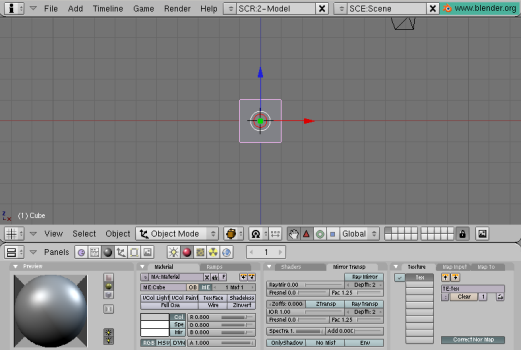
\includegraphics[scale=0.5]{oldblender.png}

\ei

\section{Starting Blender Game Engine Development}

\bi
\ii Start blender
\ii Change rendering engine from {\bf Blender Render} to {\bf Blender Game}
\ii Expand right hand panel and lower panel.
\ii Change lower panel to game logic panel.
\ei

\section{Add some objects}
\bi
\ii In the 3d window, press {\tt P}
\ii Press {\tt esc} when done
\ii Move cube up
\ii Add a material and color (original cube already has material, pick color)
\ii Snap cursor to center (shift S)
\ii Add playing surface (shift A)
\ii Go to edit mode (tab)
\ii Scale by 10 (S then 10)
\ii Exit edit mode (tab)
\ii Add a material and color (buttons on right)
\ii Press {\tt P}
\ii Press esc
\ei


\section{Add some behavior to the cube}

\bi
\ii Right-click the cube
\ii In the Game Logic panel create a keyboard sensor
\ii Set key to up arrow
\ii Create an and-controller
\ii Connect keyboard sensor
\ii Create a motion-actuator
\ii Connect and-controller
\ii Set motion to simple motion, local coordinates, change x location 9.1
\ii In 3d window, press P
\ii Press up arrow.  Cube should move forward.
\ii Press esc
\ii Add left-arrow key sensor, connect to rotate z local 1
\ii Add right-arrow key sensor, connect to rotate z local -1
\ii Play game
\ei

\section{Add some physics}

\bi
\ii Select (right click) the cube
\ii Go to physics button (bouncy ball)
\ii Change Static to Rigid Body
\ii Play game
\ii Walk off cliff
\ei

\section{Add some balls}

\bi
\ii Add Collision bounds to cube
\ii Add two spheres
\ii Give them material and color
\ii Make them rigid bodies
\ii Play game, push spheres off cliff
\ii Edit spheres, check collision sphere
\ei


\section{Using textures}

\bi
\ii In edit mode
\ii Mark seam
\ii Select all
\ii Unwrap object
\ii Go to UV editor
\ii Change View to Paint (toolbar)
\ii Use image editor or external program
\ii Make sure 3d window is in texture mode

\ei

\section{Using animations}

\bi
\ii Animate in animation screen
\ii Give animation a name
\ii Use actuator to play animation
\ii Remember to set first and last frames
\ei

\section{Character modelling}

\bi
\ii Mirror
\ei

\section{Character rigging}

\bi
\ii Set x-ray
\ii Copy/past poses in mirror form
\ei

\section{Skybox}

\bi
\ii Set material to shadeless
\ii Flip normals
\ei

\section{Miscellaneous}

\bi
\ii Press control-A to apply rotations/scales/etc.
\ei

\end{document}
